% Created 2020-05-28 jue 22:03
% Intended LaTeX compiler: pdflatex
\documentclass[11pt]{article}
\usepackage[utf8]{inputenc}
\usepackage[T1]{fontenc}
\usepackage{graphicx}
\usepackage{grffile}
\usepackage{longtable}
\usepackage{wrapfig}
\usepackage{rotating}
\usepackage[normalem]{ulem}
\usepackage{amsmath}
\usepackage{textcomp}
\usepackage{amssymb}
\usepackage{capt-of}
\usepackage{hyperref}
\author{Víctor Chico Rodríguez}
\date{\today}
\title{Referencia JAVA}
\hypersetup{
 pdfauthor={Víctor Chico Rodríguez},
 pdftitle={Referencia JAVA},
 pdfkeywords={},
 pdfsubject={},
 pdfcreator={Emacs 26.3 (Org mode 9.1.9)}, 
 pdflang={Spanish}}
\begin{document}

\maketitle
\tableofcontents

\href{./referenciajava.org}{Descargar archivo fuente .org}\\
\href{./referenciajava.pdf}{Descargar como PDF}\\
\href{./referenciajava.odt}{Descargar como OpenDocument}

\section{Introducción}
\label{sec:org8bbf8b4}
Java es un lenguage de programación orientado a objetos, fue desarrollado en 1995 por Sun MicroSystems y está basado en C++, es un lenguaje que se ejecuta en una máquina virtual que interpreta (la JVM, siglas de \emph{Java Virtual Machine}) las instrucciones compiladas a bytecode (el lenguaje de la máquina virtual). Java fue adquirido por Oracle en el año 2010.
\subsection{Estructura de un programa}
\label{sec:orgac06a28}

A lo largo de este texto veremos varios ejemplos de código fuente Java así como su salida por pantalla, a continuación un ejemplo de código Java:

\begin{verbatim}
//Este fichero pertecene al paquete (carpeta) curso.java.manual (curso/java/manual)
package curso.java.manual;

//Esto es una importación de la clase Scanner del paquete java.io
import java.io.Scanner;

//Esto es una clase pública que se llama HolaMundo
public class HolaMundo {

    /*Este es el método main (principal), 
es un método especial que servirá como punto de entrada a la aplicación. 
Este método es:
- público (puede ser accedido desde cualquier clase)
- estático (puede ser accedido sin necesidad de crear un objeto de la clase)
- no devuelve nada (tipo void)
- recibe como argumentos un array (matriz) de objetos de tipo String (cadena de texto)
*/
    public static void main (String [] args) {
	//Este es un objeto de la clase Scanner que se llama scan
	//Este objeto se inicializa con la palabra reservada new y
	//recibe como argumento System.in (Entrada del sistema)
	Scanner scan = new Scanner(System.in);

	/*
	  Esto es una llamada a un método, concretamente al método print(String)
	  del atributo out (que es un objeto de la clase PrintStream) 
	  de la clase System, este método imprime en la pantalla
	  (consola de texto) el texto que se le pase como parámetro y continúa
	  en la misma línea.
	  Como parámetro se le pasa la cadena de texto (String) "¿Cómo te llamas?"
	  Los valores de tipo String van siempre entre comillas dobles "
	 */
	System.out.print("¿Cómo te llamas? ");

	//Este es un objeto de la clase String (cadena de texto) que se llama nombre.
	//Este objeto se inicializa automáticamente con el valor que devuleve
	//el método nextString() (Método sin argumentos) del objeto scan.
	String nombre = scan.nextString();

	/*
	  Esto es otra llamada a un método, en este caso al println del atributo
	  out de la clase System, nótese la diferencia con la llamada anterior
	  (print -- println), ese ln añadido lo que hace es saltar de línea una
	  vez haya impreso lo que le pasemos como parámetro.

	  En este caso, como parámetro se le pasa una cadena de texto (igual que antes)
	  con el valor "Hola, " a lo que le concatenamos (sumamos) el valor de 
	  la variable nombre
	 */
	System.out.println("Hola, "+nombre);
    }
}
\end{verbatim}
\captionof{figure}{\label{org3adbbd2}
Hola Mundo}

Y a continuación un ejemplo de como sería su salida por pantalla si le decimos que nos llamamos Víctor:

\begin{verbatim}
¿Cómo te llamas? Víctor
Hola, Víctor
\end{verbatim}

\section{Tipos de datos}
\label{sec:org0b9a8ed}
\label{org5253f1e}
Los tipos de datos primitivos en java son los siguientes:
\begin{center}
\begin{tabular}{lll}
tipo & descripción & clase asociada\\
\hline
byte & número entero de 8 bits (-128 a 127) & Byte\\
short & número entero de 16 bits (-32768 a 32767) & Short\\
int & número entero de 32 bits (\(-2^{32}\) a \(2^{32}\)) & Integer\\
long & número entero de 64 bits (\(-2^{64}\) a \(2^{64}\)) & Long\\
float & número decimal de 32 bits & Float\\
double & número decimal de 64 bits & Double\\
boolean & valor booleano o lógico true/false (verdadero o falso) & Boolean\\
char & caracter de texto (único) & Character\\
\end{tabular}
\end{center}


Los tipos de datos normalmente se usan en su forma primitiva (columna tipo) y se pueden asignar directamente, pero a veces es util usar métodos de su clase asociada.
\section{Operadores}
\label{sec:org7f6b3a6}
\subsection{Asignación}
\label{sec:org46bc18f}
El operador \textbf{=} se usa para asignar valores a variables:
\begin{verbatim}
int a = 0;
\end{verbatim}
\subsection{Aritméticos}
\label{sec:orgd17ec59}
En java se pueden realizar multitud de operaciones matemáticas con la misma precedencia que en la vida real, si se necesita modificar se pueden utilizar paréntesis, los operadores aritméticos son los siguientes:
\begin{center}
\begin{tabular}{ll}
Operador & Descripción\\
\hline
\textbf{+} & Operador de suma\\
\textbf{-} & Operador de resta\\
\textbf{*} & Operador de multiplicación\\
\textbf{/} & Operador de división\\
\textbf{\%} & Operador de resto de la división\\
\end{tabular}
\end{center}

El siguiente código es una pequeña demostración de los operadores mencionados:

\begin{verbatim}

public class Aritmeticos {

     public static void main (String[] args) {

	 // Variable de tipo int que tendrá como valor el resultado de 1 + 2
	 int resultado = 1 + 2;
	 // El valor de resultado es 3
	 System.out.println("1 + 2 = " + resultado);
	 int resultado_original = resultado;

	 // Los operadores se pueden usar entre variables (numéricas) y números
	 // en este caso se resta 1 al valor de resultado primero y se asigna a
	 // la variable resultado después
	 resultado = resultado - 1;
	 // El valor de resultado es 2
	 System.out.println(resultado_original + " - 1 = " + resultado);
	 resultado_original = resultado;

	 // Multiplicamos el resultado por 2 y lo volvemos a asignar a la variable
	 //resultado
	 resultado = resultado * 2;
	 // El valor de resultado es 4
	 System.out.println(resultado_original + " * 2 = " + resultado);
	 resultado_original = resultado;

	 // Dividimos el resultado entre 2 y lo asignamos
	 resultado = resultado / 2;
	 // El valor de resultado es 2
	 System.out.println(resultado_original + " / 2 = " + resultado);
	 resultado_original = resultado;

	 resultado = resultado + 8;
	 // El valor de resultado es 10
	 System.out.println(resultado_original + " + 8 = " + resultado);
	 resultado_original = resultado;

	 // Dividimos el resultado entre 7 y nos quedamos con el resto, luego lo
	 // asignamos
	 resultado = resultado % 7;
	 // El valor de resultado es 3
	 System.out.println(resultado_original + " % 7 = " + resultado);
     }
 }
\end{verbatim}
\captionof{figure}{\label{org89dec8a}
Aritmeticos}

\begin{verbatim}
1 + 2 = 3
3 - 1 = 2
2 * 2 = 4
4 / 2 = 2
2 + 8 = 10
10 % 7 = 3
\end{verbatim}

Como vimos anteriormente, el operador suma \textbf{+} se puede utilizar también para concatenar texto:

\begin{verbatim}
class Concatenacion {
    public static void main(String[] args){
	String firstString = "Esto es";
	String secondString = " una cadena de texto concatenada.";
	String thirdString = firstString+secondString;
	System.out.println(thirdString);
    }
}
\end{verbatim}
\captionof{figure}{\label{org83f88a0}
Concatenación}

\begin{verbatim}
Esto es una cadena de texto concatenada.
\end{verbatim}

\subsubsection{Casteo de valores}
\label{sec:org4abfa0b}
\label{org39fc82b}
Muchas veces, cuando estamos haciendo una operación aritmética, el valor que necesitamos \emph{es más pequeño} que los posibles valores que nos puede dar como resultado la operación, con esto no queremos decir que se produzca si, por ejemplo, sumamos dos números muy grandes (ya que en ese caso, lo que podría ocurrir sería que el valor máximo del tipo de dato se excediera y \emph{diéramos la vuelta}, es decir, nos fuéramos a los números negativos, pero Java no se quejaría de esto), sino que si, por ejemplo, sumamos dos números de tipo \emph{long} y queremos guardar su resultado en una variable de tipo \emph{int}, aunque el valor de los números a sumar cupiera perfectamente en una variable de tipo \emph{int}, Java no tiene forma de saber esto, y se quejará por ello, veamos un ejemplo:

\begin{verbatim}
class ValorMuyGrande {
  public static void main(String[] args) {
    long n1 = 2;
    long n2 = 3;
    int suma = n1 + n2;
    System.out.println(suma);
  }
}
\end{verbatim}
\captionof{figure}{\label{org5f57ac9}
Valor Muy Grande}

El resultado que nos daría el compilador sería el siguiente:

\begin{verbatim}
ValorMuyGrande.java:5: error: incompatible types: possible lossy conversion from long to int
  int suma = n1 + n2;
                ^
1 error
\end{verbatim}

Es decir, Java nos está indicando que queremos meter un valor potencialmente más grande que la variable que lo va a contener, se va a producir una \emph{pérdida} en la conversión de \texttt{long} a \texttt{int}.

En los casos en los que sabemos que ese valor no excederá nuestra variable, tenemos la opción de \textbf{castear} (digamos, prometer algo a Java) que la suma devolverá un determinado tipo, esto se hace poniendo entre paréntesis el tipo de dato que devolverá una determinada función, veamos el ejemplo:

\begin{verbatim}
class ValorCasteado {
  public static void main(String[] args) {
    long n1 = 2;
    long n2 = 3;
    int suma = (int) (n1 + n2);
    System.out.println(suma);
  }
}
\end{verbatim}
\captionof{figure}{\label{org3c23f6c}
Valor Casteado}

\begin{verbatim}
5
\end{verbatim}

\subsubsection{Operadores unarios}
\label{sec:orgf52aeab}
En java hay un tipo de operadores aritméticos que sólo se utilizan en un operando, son los operadores unarios:
\begin{center}
\begin{tabular}{ll}
Operador & Descripción\\
\hline
+ & Indica un valor positivo\\
- & Indica un valor negativo\\
++ & Incrementa en 1 el valor\\
-- & Decrementa en 1 el valor\\
! & Invierte el valor de un booleano\\
\end{tabular}
\end{center}

\begin{verbatim}
class Unarios {
    public static void main(String[] args) {
	int resultado = +1;
	// El resultado es 1
	System.out.println(resultado);

	resultado--;
	// El resultado es 0
	System.out.println(resultado);

	resultado++;
	// El resultado es 1
	System.out.println(resultado);

	resultado = -resultado;
	// El resultado es -1
	System.out.println(resultado);

	boolean exito = false;
	// false
	System.out.println(exito);
	// true
	System.out.println(!exito);
    }
}
\end{verbatim}
\captionof{figure}{\label{orga058356}
Unarios}

\begin{verbatim}
1
0
1
-1
false
true
\end{verbatim}

Los operadores de incremento y decremento (\textbf{++} y \textbf{--}) actuan de manera diferente dependiendo de si se ponen delante o detrás del valor a modificar, si se usan de manera prefija \texttt{++variable} el valor se incrementa primero y la variable se usa después (ya incrementada), si se usa de manera postfija \texttt{variable++} se utilizará el valor de la variable sin incrementar y luego se incrementará:

\begin{verbatim}
class PrePost {
    public static void main(String[] args){
	int i = 3;
	i++;
	// imprime 4
	System.out.println(i);
	++i;			   
	// imprime 5
	System.out.println(i);
	// imprime 6
	System.out.println(++i);
	// imprime 6
	System.out.println(i++);
	// imprime 7
	System.out.println(i);
    }
}
\end{verbatim}
\captionof{figure}{\label{org074cb0c}
Prefijos y Postfijos}

\begin{verbatim}
4
5
6
6
7
\end{verbatim}

\subsection{Lógicos}
\label{sec:org1bc2f35}
Son operadores que devuelven valores lógicos (verdadero o falso)
\begin{center}
\begin{tabular}{ll}
Operador & Descripción\\
\hline
== & igual que\\
!= & distinto que\\
> & mayor que\\
>= & mayor o igual que\\
< & menor que\\
<= & menor o igual que\\
\&\& & Y lógico\\
\(\vert{} \vert{}\) & Ó lógico\\
instanceof & Objeto pertenece a clase\\
.equals(objeto) & Método que sirve para comparar objetos\\
\end{tabular}
\end{center}

Normalmente estos operadores se utilizarán en sentencias que requieran un valor lógico, como los condicionales o los bucles, de los que hablaremos más adelante, en este ejemplo vemos como, en base a los valores 1 y 2, que operaciones se ejecutan y cuales no:

\begin{verbatim}
class Comparacion {

    public static void main(String[] args){
	int valor1 = 1;
	int valor2 = 2;
	System.out.println ("valor1="+valor1+", valor2="+valor2);
	if(valor1 == valor2) {
	    System.out.println("valor1 == valor2 --> " + (valor1 == valor2));
	}
	if (valor1 != valor2) {
	    System.out.println("valor1 != valor2 --> " + (valor1 != valor2));
	}
	if (valor1 > valor2) {
	    System.out.println("valor1 > valor2 --> " + (valor1 > valor2));
	}
	if (valor1 < valor2) {
	    System.out.println("valor1 < valor2 --> " + (valor1 < valor2));
	}
	if (valor1 <= valor2) {
	    System.out.println("valor1 <= valor2 --> " + (valor1 <= valor2));
	}
    }
}
\end{verbatim}
\captionof{figure}{\label{orgd6e49eb}
Comparación}

\begin{verbatim}
valor1=1, valor2=2
valor1 != valor2 --> true
valor1 < valor2 --> true
valor1 <= valor2 --> true
\end{verbatim}

A veces es interesante comprobar si una comprobación cumple mas de una condición o si una sentencia se ejecutará si se cumple alguna de las condiciones posibles, es en este caso que utilizaremos los operadores lógicos \texttt{\&\&} y \texttt{||}.

\begin{verbatim}
class Condicionales {

    public static void main(String[] args){
	int valor1 = 1;
	int valor2 = 2;
	if((valor1 == 1) && (valor2 == 2))
	    System.out.println("valor1 es 1 AND (Y) valor2 es 2");
	if((valor1 == 1) || (valor2 == 1))
	    System.out.println("valor1 es 1 OR (O) valor2 es 1");
    }
}
\end{verbatim}
\captionof{figure}{\label{org031a8e4}
Operadores Condicionales}

\begin{verbatim}
valor1 es 1 AND (Y) valor2 es 2
valor1 es 1 OR (O) valor2 es 1
\end{verbatim}

\section{Condicionales}
\label{sec:org8ac4400}
En java tenemos principalmente dos estructuras condicionales, la primera es la que se compone con las sentencias \texttt{if} y \texttt{else}, y la segunda es la sentencia \texttt{switch}.

\subsection{if y else}
\label{sec:orgf850b59}
La sentencia \texttt{if} se escribe de la siguiente manera:
\begin{verbatim}
if (condicion) {
    proceso;
}
\end{verbatim}
Donde \texttt{condicion} es un valor booleano (lógico), que puede ser una variable de tipo boolean, un valor \texttt{true} o \texttt{false} directamente, aunque no tuviera mucho sentido en este caso, o el resultado de una comparación como las que acabamos de ver.

Si la condición se cumple el \texttt{proceso} (que puede ser un número indeterminado de sentencias) se ejecuta, si no se cumple, no se ejecuta, decimos que se produce un salto condicional.

Hay veces que queremos que si se cumple una condición se ejecute un determinado código y, si no se cumple, otro, esto lo conseguimos con la sentencia \texttt{else} que tiene una forma parecida al \texttt{if}, pero en este caso no se especifica condición, sino que la condición es que no se cumpla el \texttt{if}.

\begin{verbatim}
if (condicion) {
    proceso;
} else {
    otroProceso;
}
\end{verbatim}

Puede suceder que queramos comprobar una cosa y luego, independientemente otra, en ese caso solo tendríamos que tener un \texttt{if} primero y, una vez cerrado, otro con otra condición, en ese caso serían sentencias independientes y no habría ningún problema, pero podemos querer comprobar algo y, si se cumple, otra cosa después, esto lo hacemos \emph{anidando} sentencias \texttt{if} o \texttt{else}:
\begin{verbatim}
if (condicion1) {
    proceso1;
    if (condicion2) {
	proceso2;
    }
    proceso3;
} else {
    if (condicion3) {
	proceso4;
    }
}
\end{verbatim}

Si nos fijamos en el \texttt{else} (aunque esto puede ocurrir en cualquier otra parte, incluido el bloque del \texttt{if}), podemos observar que, en caso de no cumplirse la \texttt{condicion1}, podemos tener dentro otra estructura completa de sentencias \texttt{if} y cada una puede tener sus respectivos \texttt{else} y así indefinidamente, una manera de organizar mejor esté código es utilizando la sentencia compuesta \texttt{else if} que nos permite hacer varias comprobaciones sin aumentar el nivel de anidación, por ejemplo:

\begin{verbatim}
class Elseif {
  public static void main (String [] args) {
    int val = 10;
    if (val == 0) {
      System.out.println("val = 0");
    } else if (val == 1) {
      System.out.println("val = 1");
    } else if (val == 2) {
      System.out.println("val = 2");
    } else if (val == 3) {
      System.out.println("val = 3");
    } else if (val == 4) {
      System.out.println("val = 4");
    } else if (val == 5) {
      System.out.println("val = 5");
    } else {
      System.out.println("val > 5");
    }
  }
}
\end{verbatim}
\captionof{figure}{\label{orgdbe654a}
Else-If}

\begin{verbatim}
val > 5
\end{verbatim}

En este caso como el valor de la variable \texttt{val} es 10, pasaría por cada una de las condicione y, al no cumplirse, entraría por la sentencia \texttt{else} si hiciéramos esto anidando sentencias \texttt{if} y \texttt{else} el código se \emph{iría} muy a la derecha y sería más dificil de leer, pero aún tenemos otra sentencia que nos permite resolver estos problemas de una manera más elegante, la sentencia \texttt{switch}.

\subsection{switch}
\label{sec:org135fb03}

El ejemplo anterior, escrito con una sentencia switch sería el siguiente:
\begin{verbatim}
class Switch {
    public static void main (String [] args) {
      int val = 10;
      switch(val) {
      case 0:
	System.out.println("val = 0");
	break;
      case 1:
	System.out.println("val = 1");
	break;
      case 2:
	System.out.println("val = 2");
	break;
      case 3:
	System.out.println("val = 3");
	break;
      case 4:
	System.out.println("val = 4");
	break;
      case 5:
	System.out.println("val = 5");
	break;
      default:
	System.out.println("val > 5");
      }
    }
  }
\end{verbatim}
\captionof{figure}{\label{orgfe922fe}
Switch}

\begin{verbatim}
val > 5
\end{verbatim}

Como se puede observar, el código es mucho más claro, tenemos una sola sentencia condicional, \texttt{switch}, y esta, en base al valor que tenga la variable, entrará por un \texttt{case} o por otro y, en caso de que no coincida con ninguno, entrará por el \texttt{default}. Si, por ejemplo, cambiásemos el valor de \texttt{val} a 3, la salida que nos mostraría el programa sería la siguiente:

\begin{verbatim}
val = 3
\end{verbatim}

Podemos observar también una sentencia que no habíamos visto antes, la sentencia \texttt{break}, esta sentencia \emph{rompe} la ejecución del bloque en el que se encuentra, sería como ir a la llave de cierre, normalmente está desaconsejado su uso, pero en la sentencia \texttt{switch} es necesaria para cortar la ejecución donde nos interese, ya que, a diferencia de con las estructuras \texttt{if-else}, que están englobadas con llaves que nos hacen de corte, los \texttt{case} y \texttt{default} son etiquetas, y no delimitan código, lo marcan. Veamos que pasa si no ponemos la sentencia \texttt{break} en un \texttt{switch}.
\begin{verbatim}
class Switch2 {
    public static void main (String [] args) {
      int val = 2;
      //Inicializamos un contador para saber por cuantos cases pasamos;
      int contador = 0;
      switch(val) {
      case 0:
	contador++;
      case 1:
	contador++;
      case 2:
	contador++;
      case 3:
	contador++;
      case 4:
	contador++;
      case 5:
	contador++;
      case 6:
	contador++;
      case 7:
	contador++;
      case 8:
	contador++;
      case 9:
	contador++;
      case 10:
	contador++;
	System.out.println("He pasado por "+contador+" cases. El número es menor o igual que 10");
      }
    }
  }
\end{verbatim}
\captionof{figure}{\label{orgc24178e}
Switch2}

\begin{verbatim}
He pasado por 9 cases. El número es menor o igual que 10
\end{verbatim}

¿Qué ha pasado? El programa ha ejecutado todos los cases uno detrás de otro, ya que ninguno tenía una sentencia \texttt{break} para parar la ejecución y ha llegado hasta el último, donde ha imprimido el mensaje. Este ejemplo nos sirve también para ver que la etiqueta \texttt{default} no es imprescindible, como en la instrucción \texttt{if} no es imprescindible el \texttt{else}, simplemente, si no se cumple ninguna de las condiciones contempladas, no se hará nada.

\subsection{Condicional ternario}
\label{sec:org007f103}
Por último nos queda un último tipo de condicional, llamado ternario o de asignación, esta estructura nos permite asignar un valor a una variable en base al valor de otra y se escribe de la siguiente forma:

\begin{verbatim}
String miString = (condicion)?"condicion es verdadera":"condicion es falsa";
\end{verbatim}

Analizando por partes tenemos, a la izquierda del igual, una declaración de variable de tipo \texttt{String} como las que hemos visto hasta ahora, a la derecha tenemos, primero una condición lógica (del mismo tipo que las que se usan en las sentencias \texttt{if}, luego un signo de interrogación \texttt{?} que es el que nos indica que ese valor lógico no es para asignar a la variable, como hemos visto cuando asignábamos variables de tipo \texttt{boolean}, sino que es la condición para asignar la variable, el siguiente valor \texttt{"condicion es verdadera"} es el valor que tomará la variable \texttt{miString} si \texttt{(condicion)} es verdadera. Luego encontramos un signo de dos puntos \texttt{:} que separa las condiciones verdadera y falsa y, por último \texttt{"condicion el falsa"} que, como se puede intuir, es el valor que tomará \texttt{miString} si \texttt{(condicion)} es falsa.

Este condicional puede ser escrito con sentencias \texttt{if-else} de la siguiente manera (el resultado del código será el mismo):

\begin{verbatim}
String miString;
if (condicion) {
  miString = "condicion es verdadera";
} else {
  miString = "condicion es falsa";
}
\end{verbatim}

La decisión de usar una u otra dependerá de si se prefiere legibilidad del código (ternaria) o comprensión más visual (if-else).

\section{Bucles}
\label{sec:org8a36770}
La ejecució normal de un programa en java (y en casi cualquier lenguaje de programación) se hace \emph{de arriba a abajo} desde que empieza hasta que termina, los bucles son estructuras de control que permiten que una parte del código se ejecute más de una vez en base a una condición.
\subsection{El bucle while}
\label{sec:orgd8a699e}
El tipo de bucle más simple que nos encontramos es el bucle \texttt{while}, este bucle se va a ejecutar \emph{mientras} (while) la condición se cumpla y, una vez esta deje de cumplirse, seguirá desde el final del mismo.

Es importante que la condición deje de cumplirse en algún momento, y esto es válido para cualquier tipo de bucle, si la condición siempre se cumple decimos que tenemos un bucle infinito, el cual hará que nuestro programa se bloquee.

La estructura de un bucle \texttt{while} es la siguiente:
\begin{figure}[htbp]
\centering
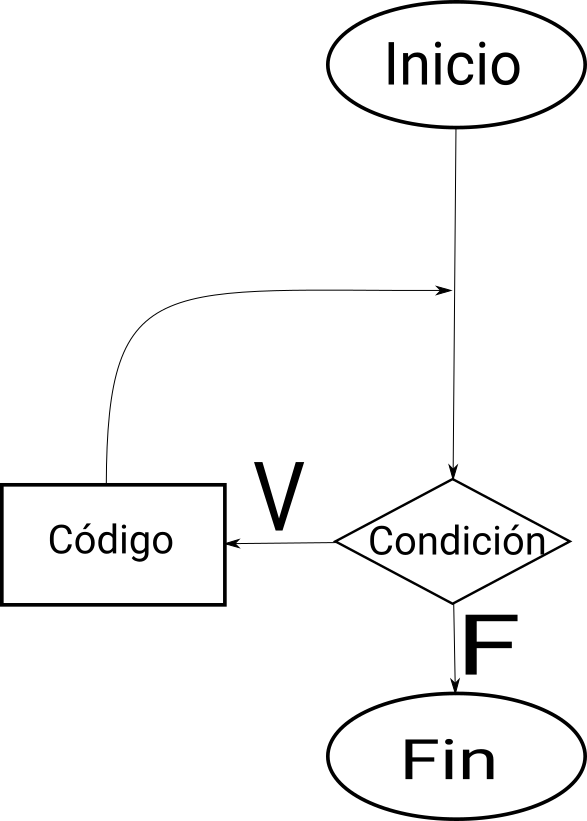
\includegraphics[width=.9\linewidth]{while.png}
\caption{Diagrama de un bucle while}
\end{figure}

Por ejemplo, si queremos un programa que muestre por pantalla los números del 1 al 10, podemos hacer lo siguiente:

\begin{verbatim}
class BucleWhile {

    public static void main(String[] args) {
	//Ponemos el número con el valor que queremos al principio
	int numeroActual=1;

	//Bucle while
	//Condición: que numeroActual sea menor o igual que 10
	while (numeroActual<=10) {

	    //Imprimimos por pantalla el número con su valor en este momento
	    System.out.println(numeroActual);

	    //Aumentamos el valor del número
	    //Si no lo hacemos, el valor de númeroActual siempre será menor o igual a 10 y tendremos un bucle infinito
	    numeroActual++;
	}
    }

}
\end{verbatim}
\captionof{figure}{\label{org5b34d13}
Bucle While}
\subsection{El bucle for}
\label{sec:orgc83896f}
\label{org916d3a3}
El bucle \texttt{for} es un caso especial del bucle \texttt{while}, este bucle se va a ejecutar igualmente mientras se cumpla la condición dada, por lo que su diagrama es el mismo, pero nos permite simplificar la programación metiendo en la cabecera tanto la inicialización de la variable como su modificación, por ejemplo, si como en el caso anterior queremos escribir los números del 1 al 10 con un bucle \texttt{for} lo haríamos así:

\begin{verbatim}
class BucleFor {

    public static void main (String[] args) {
	for (int numeroActual=1; numeroActual<=10; numeroActual++) {
	    System.out.println(numeroActual);
	}
    }

}
\end{verbatim}
\captionof{figure}{\label{org0058ee1}
Bucle For}

Como podemos ver, el resultado de este programa será exáctamente el mismo que el anterior:

\begin{verbatim}
1
2
3
4
5
6
7
8
9
10 
\end{verbatim}

La decisión de utiliar un tipo de bucle u otro depende del programador, pero se suele utiliar el bucle \texttt{for} para situaciones en las que haya que \emph{contar}, como en el caso que hemos puesto porque nos permite crear y deshechar la variable en la propia cabecera sin tener que llevar datos innecesarios, aunque por supuesto podemos usar una variable que tengamos de antes como en el bucle \texttt{while} e, incluso, no modificar la variable en la cabecera y hacerlo en el cuerpo.

\begin{verbatim}
class BucleForSinInicializacion {

    public static void main (String[] args) {
    int numeroActual=1;
    for (; numeroActual<=10; numeroActual++) {
	    System.out.println(numeroActual);
	}
    }

}
\end{verbatim}
\captionof{figure}{\label{org942f205}
Bucle For sin inicialización en la cabecera}

\begin{verbatim}
class BucleForSinModificacion {

    public static void main (String[] args) {
	for (int numeroActual=1; numeroActual<=10;) {
	    System.out.println(numeroActual);
	    numeroActual++;
	}
    }

}
\end{verbatim}
\captionof{figure}{\label{org4291339}
Bucle For Sin Modificacion en la cabecera}

Y, por supuesto, si sacamos de la cabecera tanto la inicialización como la modificación de la variable, lo que tenemos es un bucle \texttt{while} con otro nombre:

\begin{verbatim}
class BucleForSinInicializacionNiModificacion {

    public static void main (String[] args) {
	int numeroActual=1;
	for (; numeroActual<=10;) {
	    System.out.println(numeroActual);
	    numeroActual++;
	}
    }

}
\end{verbatim}
\captionof{figure}{\label{org7a0c36b}
Bucle For Sin inicialización ni Modificacion en la cabecera}

Existe un último caso de bucle \texttt{for}, se trata del también llamado bucle \texttt{for-each}, ya que sólo puede ser usado por colecciónes de elementos (no entremos en detalle ahora), y se ejecutará una vez por cada elemento de la colección, lo explicaremos en detalle más adelante pero, suponiendo una colección de elementos de tipo \texttt{String} llamada nombres su pinta sería la siguiente:

\begin{verbatim}
for (String nombre : nombres) {
  System.out.println(nombre);
}
\end{verbatim}
\captionof{figure}{Bucle \emph{for-each}}

Donde \texttt{nombre} es el nombre de la variable que vamos a usar y que va a tomar todos los valores de nuestra colección de \texttt{nombres} de uno en uno.

\subsection{El bucle do-while}
\label{sec:org1e0640c}
Hasta ahora hemos visto bucles que se ejecutan sólo si se cumple una determinada condición, pero ¿y si queremos que un fragmento de código se ejecute como mínimo una vez pero si se cumple la condición se ejecute unas cuantas mas? Podríamos duplicar el mismo código, una vez fuera del bucle y otra vez dentro, pero para ahorrarnos la reduncancia tenemos el bucle \texttt{do-while}.

Este bucle se trata de un bucle \texttt{while} en el que la condición para volverlo a ejecutar se encuentra al final y no al principio, fijémonos en el siguiente diagrama:

\begin{figure}[htbp]
\centering
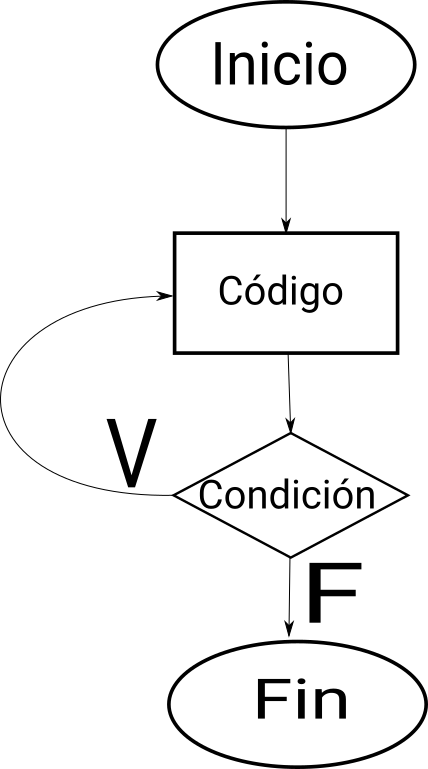
\includegraphics[width=.9\linewidth]{do-while.png}
\caption{Diagrama de un bucle do-while}
\end{figure}

Podemos continuar con nuestro ejemplo de contar de 1 a 10, veamos como se haría con un bucle do-while:

\begin{verbatim}
class DoWhile {

  public static void main(String[] args) {
    //Inicializamos la variable fuera del bucle
    int numeroActual=1;
    do {
      //Imprimimos su valor
      System.out.println(numeroActual);
      //Aumentamos la variable
      numeroActual++;
      //Comprobamos la condición, como ya se ejecuta una vez como mínimo
      //es necesario poner menor (<) y no menor o igual (<=), si lo hiciéramos
      //cuando el valor de numeroActual fuera 10 cumpliría y volvería a ejecutar
      //el código, por lo tanto contaría hasta 11
    } while (numeroActual < 10);
  }

}
\end{verbatim}
\captionof{figure}{\label{orgb685f1e}
Bucle do-while}

\begin{verbatim}
1
2
3
4
5
6
7
8
9
10 
\end{verbatim}

\section{Alcance de los elementos}
\label{sec:org077432f}
En esta sección hablaremos del ancance de los elementos, puede que programando te hayas dado cuenta de que a veces una variable que has declarado anteriormente no existe cuando la vas a utilizar más tarde, esto es porque una variable sólo está disponible desde el punto en el que se declara, si, pero además desde el bloque en el que se declara, si declaramos, por ejemplo, una variable dentro de un bloque \texttt{if}, no estará disponible fuera de este, si que podríamos declararla antes, inicializarla en el bloque \texttt{if} y entonces si estaría disponible y con el valor que le hayamos dado, el bloque más externo al que puede pertenecer una variable es el de la \textbf{clase}.

Pero existe una serie de palabras reservadas: \texttt{public}, \texttt{protected} y \texttt{private} que nos servirán para determinar como de aislada estará una determinada variable (o método, o incluso clase) en relación al resto de las clases de un programa.

Ahora hablaremos un poco de lo que significa cada una de estas palabras, no te preocupes si ahora no entiendes que quiere decir cada uno de los términos que usemos, más adelante nos ocuparemos de ello:

\begin{itemize}
\item \texttt{public}: Indica que el elemento al que se aplique estará disponible para todas las clases del programa y se puede acceder a él sin restricciones.
\item \texttt{protected}: Indica que el elemento sólo estará disponible para instancias de la clase en la que se encuentre y para clases que hereden de esta (no nos preocupemos por esta terminología ahora)
\item \texttt{private}: La variable es privada y sólo estará disponible dentro de la propia clase donde se declare.
\end{itemize}

Hay una palabra modificadora más \texttt{static} que se puede aplicar junto las demás (normalmente con \texttt{public}), esta palabra reservada nos indica que el elemento al que haga referencia estará disponible incluso sin instanciar un objeto de la clase que lo contiene (Cada vez que usas \textbf{System.out.println()}, \textbf{System} es una clase, \textbf{out} un parámetro de la misma que está declarado como \texttt{static} y \textbf{println()} un método del objeto out)
\section{Manejo de Excepciones}
\label{sec:orgbaf5793}
Inevitablemente se producirán errores en nuestro código, es un hecho, muchas veces estos errores serán \emph{en tiempo de compilación}, es decir, se producirán al tratar de compilar el código, aquí encontraremos errores de sintaxis, errores de tipos incompatibles (como el visto en el ejercicio \hyperref[org39fc82b]{Valor Muy Grande}) y cosas así, sin embargo, hay otro tipo de errores llamados de \emph{tiempo de ejecución} que solo detectaremos una vez se esté ejecutando este código, estos errores producirán que nuestro programa termine su ejecución inesperadamente y no cumpla su función, estos errores inesperados se llaman \textbf{Excepciones}.

Java lanza una \textbf{Excepción} cada vez que se produce un error de este tipo, hay excepciones de muchísimos tipos, sin entrar en detalle todavía, diremos que cada excepción es una \textbf{extensión} (una especialización) la clase \texttt{Exception}.

Veamos un ejemplo donde se lanzará una excepción:

\begin{verbatim}
class Excepciones {
  public static void main (String [] args) {
    //Creamos un objeto, un array de Strings en este caso
    String [] objeto = null;

    //En este momento, si intentamos obtener un valor de
    //este objeto, java nos dará un tipo de excepción muy concreto
    //indicando que el objeto es nulo
    objeto.toString(); 
  }
}
\end{verbatim}
\captionof{figure}{\label{orgd02d872}
Excepciones}

\begin{verbatim}
Exception in thread "main" java.lang.NullPointerException
        at Excepciones.main(Excepciones.java:9)
\end{verbatim}

\subsection{Los bloques try-catch}
\label{sec:orgd3ebdaa}
Afortunadamente Java nos proporciona una funcionalidad para capturar y controlar estos errores, se trata de los bloques \emph{try-catch}.

Los bloques \emph{try-catch} se tratan de bloques que empiezan con una sentencia \texttt{try} y dentro de ella, un bloque donde preveemos que se puede producir una excepción, seguida por uno o más bloques \texttt{catch}, cada uno de ellos encargado de \emph{capturar} una posible excepción.

Veamos un ejemplo con el anterior bloque de código:

\begin{verbatim}
class TryCatch {
  public static void main (String [] args) {
    //Creamos un objeto, un array de Strings en este caso
    String [] objeto = null;

    //Abrimos un bloque try, porque sabemos que aquí se puede
    //producir una excepción
    try {
      //En este momento, si intentamos obtener un valor de
      //este objeto, java nos dará un tipo de excepción muy concreto
      //indicando que el objeto es nulo
      objeto.toString();
    } catch(NullPointerException npe) {
      //En el bloque catch, capturamos la excepción, en este caso
      //una NullPointerException, a la que llamamos npe y que
      //dentro de este bloque podemos usar como variable.
      System.err.println("Se ha producido una NullPointerException");
    }
  }
}
\end{verbatim}
\captionof{figure}{\label{org4f483af}
Try-Catch}

\begin{verbatim}
Se ha producido una NullPointerException
\end{verbatim}

Si modificamos un poco el código anterior podemos ilustrar el hecho de que se pueden poner varios bloques \texttt{catch} en una sola sentencia \texttt{try}, a lo que añadiremos uno más, el bloque \texttt{finally}, que se ejecutará siempre, independientemente de que se produzca una excepción (y se entre en el bloque catch) o no se produzca (y, por lo tanto, no se entre en el bloque catch)

\label{org7cd0690}
\begin{verbatim}
class TryCatchMultipleFinally {
  public static void main(String[] args) {
    // Creamos un objeto, un array de Strings en este caso
    String[] objeto = null;

    // Abrimos un bloque try, porque sabemos que aquí se puede
    // producir una excepción
    try {
      // En este momento, si intentamos obtener un valor de
      // este objeto, java nos dará un tipo de excepción muy concreto
      // indicando que el objeto es nulo
      objeto.toString();
    } catch (NullPointerException npe) {
      // En el bloque catch, capturamos la excepción, en este caso
      // una NullPointerException, a la que llamamos npe y que
      // dentro de este bloque podemos usar como variable.
      System.err.println("Se ha producido una NullPointerException");
    } catch (IndexOutOfBoundsException ioobe) {
      System.err.println("Se ha producido una IndexOutofBoundsException");
    } catch (Exception e) {
      System.err.println("Se ha producido otro tipo de Excepción");
    } finally {
      System.out.println("Bloque finally");
    }

    // Inicializamos el objeto sin nada dentro
    objeto = new String[] {};

    try {
      // Intentamos obtener el primer valor del objeto
      System.out.println(objeto[0]);
    } catch (NullPointerException npe) {
      System.err.println("Se ha producido una NullPointerException");
    } catch (IndexOutOfBoundsException ioobe) {
      System.err.println("Se ha producido una IndexOutofBoundsException");
    } catch (Exception e) {
      System.err.println("Se ha producido otro tipo de Excepción");
    } finally {
      System.out.println("Bloque finally");
    }

    // Inicializamos el objeto con un valor
    objeto = new String[] {"Primer Valor"};

    try {
      // Intentamos obtener el primer valor del objeto
      System.out.println(objeto[0]);
    } catch (NullPointerException npe) {
      System.err.println("Se ha producido una NullPointerException");
    } catch (IndexOutOfBoundsException ioobe) {
      System.err.println("Se ha producido una IndexOutofBoundsException");
    } catch (Exception e) {
      System.err.println("Se ha producido otro tipo de Excepción");
    } finally {
      System.out.println("Bloque finally");
    }
  }
}
\end{verbatim}
\captionof{figure}{\label{org9af006c}
Try-Catch Múltiple y Finally}

\begin{verbatim}
Se ha producido una NullPointerException
Bloque finally
Se ha producido una IndexOutofBoundsException
Bloque finally
Primer Valor
Bloque finally
\end{verbatim}

\section{Métodos y funciones}
\label{sec:orgdfc1c3e}
Con lo que ya sabemos podemos crear programas muy potentes, podemos controlar si un bloque de código se ejecutará o no y cuantas veces lo hará, pero la ejecución sigue siendo \emph{de arriba a abajo}, estamos en lo que se conoce como \textbf{programación estructurada}, pero vayamos más allá, hasta ahora, si queríamos ejecutar un bloque de código más de una vez podíamos hacer bucles, pero estos siempre se ejecutarán con los mismos datos, la estructura de un método es la siguiente:

\begin{verbatim}
public static void main (String [] args)
\end{verbatim}
\captionof{figure}{Estructura de un método}

\begin{itemize}
\item En azul vemos los modificadores, no nos pararemos ahora a explicarlos en detalle, digamos que es un método público (que puede ser accedido desde cualquier clase) y estático (que puede ser accedido sin necesidad de crear una instancia del método)
\item En rojo tenemos el \emph{tipo de retorno}, puede ser cualquiera de los tipos de dato conocidos (int, char, long, boolean\ldots{}), cualquier tipo de clase (como por ejemplo, String), o \texttt{void}, que significa que el método no devolverá nada.
\item En morado vemos el nombre del método, es el que utilizaremos para invocarlo
\item A continuación tenemos los paréntesis, en estos paréntesis irán los parámetros que entrarán al método, declarados de la misma manera que se hace con las variables (tipo de variable seguido del nombre de la variable), separados por comas, o bien nada, con el paréntesis vacío si el método no necesita parámetros.
\end{itemize}

Hay un tipo de paso de parámetros un poco especial, conocido como \emph{varargs}, que consiste en que un método recibirá un número indeterminado de parámetros de un tipo, se escribe poniendo tres puntos detrás del tipo de variable, antes del espacio y el nombre y solo puede ser usado una vez por método y al final de la lista de parámetros. Como ilustración, este tipo de parámetro se escribe de la siguiente manera:

\begin{verbatim}
public String varargs(String... parametros)
\end{verbatim}
\captionof{figure}{Varargs}

Esa variable \texttt{parametros} que tenemos en el ejemplo anterior, se accederá como si fuera un objeto de tipo array del tipo que se indique (en este caso String).

Veamos ahora un ejemplo sencillo de la potencia de un método con el que podemos ejecutar un mismo código con \textbf{parámetros} diferentes:

\begin{verbatim}
class MiPrimerMetodo {

  //Aquí tenemos el método main, no devuelve nada (void)
  //y recibe como parámetro un array de Strings (varias cadenas de texto)
  public static void main(String [] args) {
    //Creamos una variable llamada nombre y la inicializamos
    String nombre = "Bimo";
    //Llamamos a nuestro método y le pasamos como parámetro la variable
    saludar(nombre);
    //Cambiamos el valor de la variable
    nombre = "Kirby";
    //Y volvemos a llamar al método
    saludar(kirby);
  }

  //Aquí tenemos nuestro método, se llama saludar y no devuelve nada,
  //recibe como parámetro una cadena de texto llamada nombre,
  //cada vez que se ejecute saludará a quien venga escrito en la variable nombre
  static void saludar(String nombre) {
    System.out.println("Hola, "+nombre);
  }

}
\end{verbatim}
\captionof{figure}{\label{orgd927121}
Mi primer método}

\begin{verbatim}
Hola, Bimo
Hola, Kirby
\end{verbatim}

\subsection{Paso de parámetros}
\label{sec:org719c346}
En el ejemplo anterior hemos visto que al método \emph{saludar} le pasábamos un parámetro, un nombre en este caso, de tipo String, cuando declaramos un método, dentro de los paréntesis le podemos poner, separados por comas, todos los parámetros que vaya a necesitar para cumplir su función, estos parámetros se escriben de la misma manera que se creaban las variables (pero sin inicializar), y cuando se les invoca se le pasan las variables necesarias que se correspondan con los parámetros que requiere, veamos un ejemplo:

\begin{verbatim}
//Supongamos que llegamos a este método,
//como se ve, no tiene parámetros ni devuleve nada (void)
public void metodo1() {
  System.out.println("El número es: "+metodo2());
}

//Este método es privado, sólo se puede invocar desde
//esta clase, y devuelve un número entero,
//tampoco recibe parámetros
private int metodo2() {
  int numero = metodo3(2);
  return numero;
}

//Este es otro método privado, que recibe como
//parámetro un número entero y llama al metodo4
private int metodo3(int numero) {
  return metodo4(numero, 0.5);
}

//Este método recibe como parámetros un número entero
//y un número decimal y los multiplica, después devuleve
//el resultado entero.
private int metodo4(int numero, double factor) {
  return (Integer)(numero * factor);
}
\end{verbatim}

En Java, se dice que los parámetros que se pasan a los métodos se hacen \emph{por valor}, esto quiere decir que cada método hace una copia del parámetro cuando se invoca y, se asignamos un nuevo valor al parámetro dentro del método, este no cambiará en el método que lo invocó, veamos un ejemplo:

\begin{verbatim}
class PasoDeValor {

  //Declaramos un método al que llamaremos,
  //Como podemos ver, podemos declararlo antes
  //del método main, aunque se le llamará después
  static void cambiarValor(int numero) {
    numero = 2;
  }

  public static void main (String [] args) {
    //Declaramos una variable y le asignamos un valor
    int numero = 1;

    //Llamamos al métod de cambio de valor
    cambiarValor(numero);

    //Mostramos el resultado por pantalla
    System.out.println(numero);
  }

}
\end{verbatim}
\captionof{figure}{\label{orgc1af153}
Paso de valor}

\begin{verbatim}
1
\end{verbatim}

Se puede pensar que el que los valores no pasen de los métodos a quien los llamó es poco util, pero si puede hacerse, para ello usaremos la sentencia \textbf{return}, que literalmente \emph{devuelve} el valor que le digamos, si modificamos un poco el programa anterior lo veremos:

\begin{verbatim}
class RetornoDeValor {

  //Declaramos un método al que llamaremos,
  //Como podemos ver, podemos declararlo antes
  //del método main, aunque se le llamará después.
  //En este caso hemos cambiado el tipo de retorno del método
  // de void (no devuleve nada) a int, y hemos añadido la sentencia
  // return con nuestra variable.
  static int cambiarValor(int numero) {
    numero = 2;
    return numero;
  }

  public static void main (String [] args) {
    //Declaramos una variable y le asignamos un valor
    int numero = 1;

    //Llamamos al métod de cambio de valor
    //y le asignamos el valor del retorno
    numero = cambiarValor(numero);

    //Mostramos el resultado por pantalla
    System.out.println(numero);
  }

}
\end{verbatim}
\captionof{figure}{\label{orge947016}
Retorno de valor}

\begin{verbatim}
2
\end{verbatim}

Ahora, para ver otra característica del paso de parámetros a los métodos, tenemos que hacerlo mediante objetos, de momento no nos preocupemos mucho de ello, básicamente lo que tenemos que tener en cuenta es que si pasamos un objeto como parámetro y cambiamos el valor de una de sus propiedades dentro de un método, esta permanecerá cambiada incluso fuera del método, esto puede parecer lo opuesto a lo que acabamos de ver, pero no es así, si en lugar de cambiar el valor de una de las propiedades del objeto lo que hiciéramos fuera instanciar un nuevo objeto en la variable (como asignar un nuevo valor en las variables que ya conocemos), el valor de la variable original permanecería intacto, veamoslo de nuevo con dos ejemplos:

\begin{verbatim}
import java.util.ArrayList;

class CambioDeObjeto {
  public static void main (String [] args) {
    /*
      Creamos un objeto de tipo ArrayList, este objeto consiste un una lista del tipo de objetos
      que le digamos entre los acentos, en este caso Integer (número entero), se declara como ya
      sabemos TipoDeObjeto nombreDeLaVariable, y luego se le asigna un valor, en este caso, un objeto
      nuevo de la clase ArrayList, los paréntesis que aparecen al final son porque estamos llamando
      al método constructor del objeto, sin parámetros en este caso, aunque puede haberlos.
     */
    ArrayList<Integer> lista = new ArrayList<Integer>();

    /*
      Añadimos un objeto de la clase Integer (un 1), en el objeto lista, para ello llamamos al método
      add de la clase ArrayList, con un parámetro de tipo entero (el 1), este método añade un objeto a      la lista.
     */
    lista.add(1);

    //Imprimimos el valor del primer elemento de la lista (posición 0), llamando al método get de la clase ArrayList
    System.out.println(lista.get(0));
  }

  /*
    Se asigna un nuevo valor a la variable lista 
   */
  static void nuevoObjeto(ArrayList<Integer> lista) {
    lista = new ArrayList<Integer>();
    lista.add(2);
  }
}
\end{verbatim}
\captionof{figure}{\label{orga62e502}
Cambio de objeto}

\begin{verbatim}
1
\end{verbatim}

Ahora vamos a ver como podemos añadir un valor al objeto que ya existe

\begin{verbatim}
import java.util.ArrayList;

class CambioDePropiedad {
  public static void main (String [] args) {
    /*
      Creamos un objeto de tipo ArrayList, este objeto consiste un una lista del tipo de objetos
      que le digamos entre los acentos, en este caso Integer (número entero), se declara como ya
      sabemos TipoDeObjeto nombreDeLaVariable, y luego se le asigna un valor, en este caso, un objeto
      nuevo de la clase ArrayList, los paréntesis que aparecen al final son porque estamos llamando
      al método constructor del objeto, sin parámetros en este caso, aunque puede haberlos.
     */
    ArrayList<Integer> lista = new ArrayList<Integer>();

    //Llamamos al método para asignar un nuevo valor a la propiedad
    anadirValor(lista);

    /*
      Añadimos un objeto de la clase Integer (un 1), en el objeto lista, para ello llamamos al método
      add de la clase ArrayList, con un parámetro de tipo entero (el 1), este método añade un objeto a la lista.
      En este caso, se añadirá en la posición 1 (la segunda).
     */
    lista.add(1);

    //Imprimimos el valor del primer elemento de la lista (posición 0), llamando al método get de la clase ArrayList
    System.out.println(lista.get(0));
  }

  /*
    Se asigna un nuevo valor a la variable lista
   */
  static void anadirValor(ArrayList<Integer> lista) {
    lista.add(2);
  }
}
\end{verbatim}
\captionof{figure}{\label{org590a06d}
Cambio de propiedad}

\begin{verbatim}
2
\end{verbatim}

\subsection{Sobrecarga de métodos}
\label{sec:org0ef0371}
Expliquemos ahora un nuevo concepto, se trata de la \emph{sobrecarga de métodos}, una función extremádamente útil que tiene Java, a pesar del nombre tan rimbombante que tiene se trata simplemente de la posibilidad de tener un método con el mismo nombre pero con diferentes parámetros, sean o bien diferente número o diferente tipo (o ambas, obviamente).

La forma que tiene Java de permitir esto es asignando a cada método una \emph{firma}. La firma de un método viene dada por su nombre y los tipos de sus atributos, es importante porque en una misma clase \textbf{no puede haber dos o más métodos con la misma firma}. Veamos un ejemplo:

\begin{verbatim}
class SobrecargaDeMetodos {

  public static void main (String[] args) {

    saludar("Víctor");
    saludar("Víctor","Toledo");
    saludar(30);
    saludar("Víctor",30);
    saludar("Víctor","Toledo",30);
    saludar();

  }

  static void saludar(String nombre) {
    System.out.println("Hola, "+nombre+". No se tu edad ni donde naciste :(");
  }

  static void saludar(String nombre, String ciudad) {
    System.out.println("Hola, "+nombre+", no se tu edad, pero se que naciste en "+ciudad);
  }

  static void saludar(int edad) {
    System.out.println("Hola, no se como te llamas ni donde naciste, pero se que tienes "+edad+" años");
  }

  static void saludar(String nombre, int edad){
    System.out.println("Hola, "+nombre+", naciste hace "+edad+" pero no se dónde");
  }

  static void saludar(String nombre, String ciudad, int edad) {
    System.out.println("Hola "+nombre+"! Te conozco bien, tienes "+edad+" años y naciste en "+ciudad);
  }

  static void saludar() {
    System.out.println("Hola, no te conozco en absoluto, no se ni tu edad, ni dónde naciste :'(");
  }

}
\end{verbatim}
\captionof{figure}{\label{org8865727}
Sobrecarga de métodos}

\begin{verbatim}
Hola, Víctor. No se tu edad ni donde naciste :(
Hola, Víctor, no se tu edad, pero se que naciste en Toledo
Hola, no se como te llamas ni donde naciste, pero se que tienes 30 años
Hola, Víctor, naciste hace 30 años pero no se dónde
Hola Víctor! Te conozco bien, tienes 30 años y naciste en Toledo
Hola, no te conozco en absoluto, no se ni tu edad ni dónde naciste :'(
\end{verbatim}

Fijémonos ahora en las firmas de las diferentes sobrecargas del método \emph{saludar}
\begin{enumerate}
\item saludar(String)
\item saludar(String, String)
\item saludar(int)
\item saludar(String, int)
\item saludar(String, String, int)
\item saludar()
\end{enumerate}

Podemos ver que en las firmas a Java \emph{le da igual} el nombre de los parámetros, solo le importa su tipo, esto nos limita a que, por ejemplo no podríamos tener un método con que nos saludase con la ciudad de nacimiento y la edad de la siguiente forma:

\begin{verbatim}
static void saludar(String ciudad, int edad){
\end{verbatim}

Ya que tendría la misma firma que el método \textbf{4} \emph{saludar(String, int)}, no obstante si que podríamos haberlo añadido de la siguiente manera:

\begin{verbatim}
static void saludar(int edad, String ciudad){
\end{verbatim}

Ya que aquí el método tendría una firma que sería \emph{saludar(int, String)}, que no coincide con ninguna de las otras 6.

\subsection{Recursividad}
\label{sec:orgb60e5b8}
Otra de las cosas a las que no da acceso un método es el concepto de la \emph{recursividad}, esto no es más que un método que se llama a si mismo, por lo tanto tendremos que parar esas llamadas cuando se cumpla una determinada condición como ocurría con los bucles o tendremos un bucle de recursividad infinito y nuestro programa no avanzará.

Un ejémplo clásico de recursividad es el cálculo de un factorial, pero ántes veamos como sería diseñar el cálculo de un factorial con un bucle.

\begin{center}
El factorial de un número se define como la multiplicación de si mismo con todos sus números anteriores. Por ejemplo el factorial de 6 ó \textbf{6!} = 6*5*4*3*2*1, una de las principales razones de que el factorial se use como ejemplo para la recursividad en programación es que el factorial ES recursivo, si vemos, por ejemplo el factorial de 5 (\textbf{5!}) = 5*4*3*2*1, si se compara con 6! como hemos visto antes vemos un patrón, y es que 6! = 6*5!, y así sucesivamente.
\end{center}

\begin{verbatim}
private static long factorialLoop (int n) {
    long resultado = 1;
    while (n>1) {
	resultado *= n--;
    }
    return resultado;
}
\end{verbatim}
\captionof{figure}{Factorial con bucle}

El método anterior recibe un número entero y si es mayor que 1 va multiplicando el resultado por el número \texttt{n} y reduce su valor en 1 hasta que es 1 y sale del bucle.

A continuación el mismo método utilizando recursividad, se puede observar que es bastante similar, pero conceptualmente es más coherente con la definición del factorial:

\begin{verbatim}
private static long factorialRecur (int n) {
    long resultado=1;
    if (n > 1) {
       resultado = n*factorialRecur (n-1);
    }
    return resultado;
}
\end{verbatim}
\captionof{figure}{Factorial con recursividad}

En este caso se entra al método y si n es mayor que 1 se multiplica su valor por el resultado de llamarse a si mismo decrementando en 1 el valor de n. Conviene saber aquí que java, ante una operación da preferencia a la llamada de un método, por ejemplo, la traza de llamar al método \texttt{factorialRecur(4)} sería algo similar a lo siguiente:

\begin{center}
entramos en  factorialRecur(4) -> entramos en factorialRecur(3) -> entramos en factorialRecur(2) -> entramos en factorialRecur(1) -> factorialRecur(1) devuelve 1 -> factorialRecur(2) multiplica 2*1 y devuelve 2 -> factorialRecur(3) multiplica 3*2 y devuelve 6 -> factorialRecur(4) multiplica 4*6 y devuelve 24
\end{center}

Es decir, el método recursivo va \emph{bajando} por las llamadas hasta llegar a lo que se llama \textbf{caso base}, en este caso el factorial de 1, que es 1 (aunque lo correcto hubiera sido llegar hasta 0!, que también es 1, pero el resultado es el mismo) y después, según los métodos van llegando a su sentencia \texttt{return} vuelve a \emph{subir} hasta el caso de la primera llamada (factorialRecur(4) en nuestro caso).

\section{Clases y objetos}
\label{sec:org94e4ebe}
Como ya hemos comentado anteriormente, Java es un lenguaje de programación \emph{orientado a objetos}, en Java, prácticamente todo es un objeto, salvo los tipos de datos primitivos (int, char, boolean,\ldots{}) que incluso también tienen una clase asociada (Integer, Character y Boolean, respectivamente para los ejemplos anteriores, nótese que empiezan por mayúscula), aunque probablemente, la clase con la que estarás más familiarizada será la clase String, usada para cadenas de texto.

Muchas veces se usan indistintamente los términos clase y objeto, lo correcto es llamar clase al archivo fuente .java y objeto a las \emph{instancias} de este.

\subsection{El método constructor}
\label{sec:org3e87e2e}
En Java (y en cualquier otro lenguaje de programación orientado a objetos), llamamos instanciar al hecho de crear un objeto de una determinada clase en nuestro código, para ello hacemos uso de un tipo de método especial llamado \textbf{constructor}.

Este método es especial por varios motivos:

\begin{enumerate}
\item Es un método sin nombre, su nombre es el nombre de la propia clase
\item Es necesario invocarlo unido a la palabra reservada \textbf{new}
\end{enumerate}

Esto lo hemos visto anteriormente en el ejemplo de paso de variables por valor a los métodos de la siguiente manera:

\begin{verbatim}
ArrayList<Integer> lista = new ArrayList<Integer>();
\end{verbatim}

Analizando la sentencia anterior tenemos lo siguiente:
\begin{itemize}
\item ArrayList<Integer>: El tipo de objeto que vamos a crear, exáctamente igual que cuando creábamos variables de tipo int, char, boolean, String,\ldots{}. En este caso, un objeto ArrayList (Un tipo de lista) de objetos de tipo Integer (o int, números enteros)
\item lista: El nombre de la variable, nada nuevo aquí.
\item new ArrayList<Integer>(): y aquí tenemos la llamada al método constructor, como podemos ver, es un método que se llama igual que la clase que queremos instanciar (ArrayList<Integer>) y que va seguido por unos paréntesis, en este caso, sin nada dentro porque no le pasamos ningún parámetro, todo ello precedido de la palabra reservada \textbf{new}, que es la que le indica a Java que lo que venga detrás será un método constructor.
\end{itemize}

En Java, por convención, las clases empiezan con mayúscula, meintras que los nombres de las variables y los métodos se escriben empezando con minúscula, en ambos casos siguiendo la convención \emph{CamelCase} (\emph{UpperCamelCase}, comenzando con mayúscula para las clases y \emph{lowerCamelCase}, comenzando con minúscula para lo demás), que consiste en, si necesitamos varias palabras en el nombre, separarlas con mayúsculas y sólo usarlas en ese caso o en caso de abreviaturas conocidas, por ejemplo, podríamos tener un método que se llamase \emph{getSQL}, ya que \emph{SQL} es una abreviatura bien conocida.

\subsection{El caso de la clase String}
\label{sec:org1610774}

Anteriormente hemos instanciado una clase que es un caso especial, no lo hemos hecho mediante un método constructor, sino asignándole un valor con = como hacíamos con los tipos primitivos, se trata de la clase String.

Esta clase, por ser tan extendida se crea de esta manera, que nos puede dar la impresión de que se trata de un tipo de variable primitivo:

\begin{verbatim}
String nombre = "Kirby";
\end{verbatim}

Pero en realidad lo que estábamos haciendo era crear una nueva instancia (un nuevo objeto) de la clase String.

La clase String, como cualquier otra clase en Java necesariamente debe tener al menos un método constructor, y así es, es sólo que Java nos ofrece esta conveniencia.

\subsection{El valor null}
\label{sec:org9f0be17}
Hasta ahora, cuando creábamos una variable esta podía estar inicializada o no, y, si lo estaba, tenía un valor válido dentro de su tipo, el valor \textbf{null} es un valor especial, nos permite indicar que el contenido de una variable de tipo objeto es nulo, es decir, no contiene nada pero existe como variable, el valor \textbf{null} es el mismo para cualquier tipo de objeto, se puede asignar a cualquier objeto con el operador de asignación (=) y puede ser usado en operaciones de comparación, vamos a ver un ejemplo:

\begin{verbatim}
class ValorNull {
  public static void main(String [] args) {

    //Asignamos el valor null a una objeto instancia de la clase String
    String nombre = null;

    //Comprobamos si la variable nombre es nula (valor null)
    if (nombre == null) {
      nombre = "Kirby";
    }

    System.out.println(nombre);

  }
}
\end{verbatim}
\captionof{figure}{\label{orgb2772cb}
Valor null}

\begin{verbatim}
Kirby
\end{verbatim}

\subsection{Clases más conocidas}
\label{sec:org9906d68}
\subsubsection{La clase Object}
\label{sec:orgf9b764f}
En Java todos los objetos que exiten, ya sean los que nos proporciona el propio lenguaje o los que creemos nosotros extienden de la clase \texttt{Object}. Object es la clase primaria del lenguaje de programación Java, no se usa mucho como tal, pero es conveniente conocer que existe, podemos declarar un objeto de esta clase e instanciarlo con cualquier otra, es la madre de todas las demás.

\subsubsection{String}
\label{sec:org94bb8f8}
Como acabamos de ver, la clase String probablemente sea la clase más conocida de Java, empezamos a trabajar con ella prácticamente en el primer programa HolaMundo que hacemos y la utilizamos tanto como a los tipos primitivos, sirve para guardar cadenas de texto y no nos detendremos mucho más en ella.

\begin{enumerate}
\item Métodos
\label{sec:orge132bd3}
\begin{itemize}
\item equals(objeto): Aunque este método es genérico para todos los objetos, es importante recalcarlo, ya que muchas veces querremos comparar si una cadena de texto es igual a otra.
\item equalsIgnoreCase(objeto): Este método es igual que el anterior salvo que ignora las mayúsculas y las minúsculas.
\item charAt(indice): Devuelve la letra (como tipo \texttt{char}) que haya en el índice que le pasemos.
\item length(): Nos devuelve el tamaño del texto.
\item indexOf(cadena): nos devuelve la primera posición en la que aparece la cadena.
\item lastIndexOf(cadena): igual que el anterior, pero nos devuelve la última.
\item toUpperCase(): Convierte la cadena en mayúsculas.
\item toLowerCase(): Convierte la cadena en minúsculas.
\item valueOf(objeto): Método estático que devuelve el valor del objeto en forma de string.
\end{itemize}
\end{enumerate}

\subsubsection{Clases asociadas a tipos primitivos}
\label{sec:org23c75e6}
Como ya vimos en la sección \hyperref[org5253f1e]{Tipos de datos}, los tipos primitivos tienen una clase asociada a cada uno de ellos, el nombre del tipo de dato es normalmente una abreviatura del nombre completo de la clase y se escribe en minúscula, mientras que la clase, como hemos visto antes, se escribirá en mayúscula. Estas clases son especialmente útiles, ya que, además de contener una serie de métodos que nos ofrecen funciones para trabajar con estos tipos de datos, pueden ser usados para almacenar el valor \textbf{null} en ellos, indicando así que un dato que normalmente tendría un valor por defecto, no contiene nada.

\begin{enumerate}
\item Métodos
\label{sec:org2581e17}
Uno de los métodos más importantes de estas clases es el método estático parse\ldots{}(cadena), los puntos suspensivos son porque su nombre es diferente para cada clase, por ejemplo Long.parseLong() para la clase Long, Integer.parseInt() para la clase Integer, etc., este método convierte una cadena en el tipo que haga referencia, es especialmente útil cuando queremos que un usuario nos introduzca un valor por la consola, ya que siempre llegará en forma de String y si lo que necesitamos es un número deberemos convertirlo de esta manera.
\end{enumerate}

\subsubsection{Matrices (o Arrays)}
\label{sec:org1144f14}
Las matrices (o Arrays, como se llaman en inglés y, comunmente en los entornos de trabajo) pertenecen a un grupo de objetos que se conocen como \textbf{colecciones}, estas colecciones consisten en una agrupación de varios objetos, en el caso de los arrays, una lista. Los arrays lo pueden ser de cualquier tipo de objeto (pero sólo de uno a la vez) y se identifican porque se declaran con el nombre del tipo del que queremos la lista y unos corchetes \texttt{[]}.

Para insertar o recoger los valores de la lista lo haremos llamando a la variable como hacíamos habitualmente y añadiendo un número entre corchetes, como vimos en el ejercicio \hyperref[org7cd0690]{TryCatchMultipleFinally}, en ese ejercicio intentábamos obtener el primer valor (índice 0) de la variable \texttt{objeto} y lo hacíamos de la siguiente manera:

\begin{verbatim}
objeto[0];
\end{verbatim}

Esa simple instrucción nos apunta a la primera posición del array, hay que tener en cuenta que los arrays, como la gran mayoría de estructuras múltiples que existen en los lenguajes de programación, se empiezan a contar desde 0 y no desde 1, es decir, en un array con un tamaño de 5, las posiciones a las que podemos acceder son las 0, 1, 2, 3 y 4; si intentásiemos acceder a la posición 5, Java nos lanzaría una \texttt{IndexOutOfBoundsException} como vimos en el ejercicio mencionado anteriormente. Esta excepción nos indica que hemos intentado acceder a un índice (posición) más allá de los límites del objeto (El objeto tiene 5 posiciones y hemos intentado acceder a la 6ª).

Una vez tenemos una posición que existe, podemos asignarle un valor o recogerlo como hacíamos con cualquier otro tipo de variable. Para ilustrarlo:

Igual que hacíamos:

\begin{verbatim}
class AccesoVariable {
  public static void main (String [] args) {
    int numero; //Declaramos la variable
    numero = 2; //inicilizamos la variable
    System.out.println(numero); //Obtenemos el valor de la variable
  }
}
\end{verbatim}
\captionof{figure}{\label{orgb10171d}
Acceso a variable}

\begin{verbatim}
2
\end{verbatim}

Podemos hacer:

\begin{verbatim}
class AccesoArray {
  public static void main (String [] args) {
    int[] array; //Declaramos la variable
    array = new int[]{2}; //Inizializamos la variable (con un valor en la posición 1)
    System.out.println(array[0]); //Obtenemos el valor de la posición 1
  }
}

\end{verbatim}
\captionof{figure}{\label{orgd8ef8cb}
Acceso a posición de array}

\begin{verbatim}
2
\end{verbatim}

\begin{enumerate}
\item Declaración e inicialización
\label{sec:org214ef95}
Como todos los objetos, los arrays pueden ser inicializados con la palabra reservada \texttt{new} y llamando al constructor, pero esta clase, al igual que la clase \texttt{String} es una clase especial y puede ser inicializada de varias maneras.

\begin{enumerate}
\item Inicialización con constructor vacío
\label{sec:org5ef2a80}
En este caso lo haremos de la siguiente manera, por ejemplo, para un array de números enteros (int o Integer):

\begin{verbatim}
int[] miArray = new int[5];
\end{verbatim}
\captionof{figure}{Inicialización de un array con constructor}

Observamos que también se trata de un caso especial (no hay paréntesis en la llamada al método constructor), de izquierda a derecha, lo que tenemos es:

\begin{itemize}
\item Antes del \texttt{=}:
\begin{itemize}
\item int[]: Tipo de dato, array ([]) de números enteros (int).
\item miArray: El nombre de la variable.
\end{itemize}
\item Después del \texttt{=}:
\begin{itemize}
\item new: La palabra reservada que nos indica que lo que queremos es invocar al método constructor.
\item int[5]: La llamada propiamente dicha, el número que vemos entre los corchetes será el tamaño de la lista, hemos de tener en cuenta que este tamaño es fijo, por lo que no nos conviene quedarnos cortos, pero sería un desperdicio de memoria si nos pasamos, es un valor que hay que pensar muy bien.
\end{itemize}
\end{itemize}

Ahora ya podríamos añadir valores a nuestro array, por ejemplo, añadamos un 2 en la posición 4:

\begin{verbatim}
miArray[3] = 2;
\end{verbatim}
\captionof{figure}{Añadir valor a array}

\item Inicialización con constructor con datos
\label{sec:orge017584}
El caso anterior, aunque util de conocer, en ocasiones nos parecerá engorroso, pues tendremos que rellenar el array escribiendo una sentencia para cada posición que tenga, afortunadamente, en Java se puede inicializar el array directamente en el constructor de la siguiente manera:

\begin{verbatim}
int[] miArray = new int[]{5,4,3,2,1};
\end{verbatim}
\captionof{figure}{Array con datos}

De esta manera no nos hace falta indicarle al constructor cuantos elementos tendrá el array, en cambio, le decimos los valores en orden que almacenará (en nuestro caso; 5 en la posción 1, 4 en la posición 2, 3 en la posición 3, etc.)

\item Inicialización con datos sin constructor
\label{sec:org52e8e60}
Este es el caso más especial, y es que podemos evitar escribir la parte del constructor y poner solo las llaves con los datos si lo hacemos justo cuando declaremos la variable:

\begin{verbatim}
int[] miArray = {5,4,3,2,1};
\end{verbatim}
\captionof{figure}{Array con datos sin constructor}

Si lo quisiéramos separar de la declaración, este formato daría error, ya que Java no tiene manera de asegurarse de qué tipo es lo que queremos asignar a la variable, en este caso habría que usar el constructor anterior:

\begin{verbatim}
int[] miArray;

miArray = {5,4,3,2,1}; //Esto da error

miArray = new int[]{5,4,3,2,1}; //Esto funciona
\end{verbatim}
\captionof{figure}{Declaración separada}
\end{enumerate}

\item Arrays múltiples
\label{sec:orgd4605c3}
Otra cosa interesante que nos permiten hacer los arrays es añadir unos dentro de otros, obteniendo así estructuras \emph{multidimensionales}.

Si entendemos que un array \texttt{[]} es una lista (o una línea de valores, si queremos), si cada elemento del array es otro array \texttt{[][]} lo que tenemos es un cuadro y, si a su vez, cada elemento del cuadro es otra matriz \texttt{[][][]} lo que tenemos es un cubo de valores y, para acceder a cada uno de ellos es necesario indicar cada una de las coordenadas que indican su posición.

Los arrays multidimensionales se comportan exáctamente igual que los planos, sólo hay que tener en cuenta las dimensiones extra para tener claro a qué valor estamos accediendo, que para inicializarlos es necesario indicar el tamaño de cada uno de las dimensiones (no tienen por qué ser regulares) y que si queremos inicializarlo directamente con valores, cada elemento que va entre las comas dentro de las llaves serán a su vez otras llaves hasta que se haya profundizado en cuantas dimensiones tenga, por ejemplo, un array multidimensional lo podríamos instanciar así:

\begin{verbatim}
int[][] miArrayMultidimensional = new int[3][12];

String[][] otroArrayMultidimendional = {{"p11","p12","p13"},{"p21","p22","p23"}};
\end{verbatim}
\captionof{figure}{Array Multidimensional}
\item Métodos y propiedades
\label{sec:orga3be728}
\begin{itemize}
\item lentgh: propiedad que nos indica la longitud del array
\end{itemize}
\item Recorriendo un Array
\label{sec:org3271345}
Dada su naturaleza, muchas veces nos interesará recorrer todos los valores de un array, ya sea para buscar un valor concreto si no sabemos su posición, para imprimir todos los valores o para cualquier otra cosa que se nos pueda ocurrir. Esto se puede conseguir de múltiples maneras, pero las más común sería utilizando un \hyperref[org916d3a3]{bucle \textbf{for}}.

Por ejemplo, si tenemos el siguiente Array de Strings

\begin{verbatim}
String[] nombres = {"Pepe","Juan","María","Beatriz","Víctor","Raquel"};
\end{verbatim}

Podríamos hacer un bucle for clásico para recorrer e imprimir cada uno de los valores del array:

\begin{verbatim}
//Nuestro bucle for recorrerá desde la posición 0, hasta la última del array
//identificada por su propiedad length y sumará 1 a la variable i en cada
//iteración del bucle
for (int i=0; i<nombres.length; i++) {
  System.out.println("Hola, "+nombres[i]);
}
\end{verbatim}

Pero como vimos en la sección dedicada al bucle for, teníamos un tipo de bucle que se ejecuta una vez por cada elemento de una colección y, efectivamente, un array es una colección de elementos como habrás podido deducir. Por lo tanto, usando esta manera simplificaremos el bucle:

\begin{verbatim}
for (String nombre : nombres) {
  // Ya no tenemos una variable i con la que acceder a cada posición del array nombres (nombres[i])
  // sino que tenemos una variable nombre, del mismo tipo que cada elemento del array, en este caso
  // de tipo String, que en cada iteración contendrá el un valor del array de nombres
  System.out.println("Hola, "+nombre);
}
\end{verbatim}

En ambos casos el resultado será el mismo:

\begin{verbatim}
Hola, Pepe
Hola, Juan
Hola, María
Hola, Beatriz
Hola, Víctor
Hola, Raquel
\end{verbatim}
\end{enumerate}

\subsubsection{Date}
\label{sec:org11fd397}
La clase Date del paquete java.util es una clase que nos permite almacenar fechas.

\begin{enumerate}
\item Declaración e inicialización
\label{sec:org8c4fd47}
Como cualquier objeto, la clase Date se inicializa a través de la palabra reservada \texttt{new}:

\texttt{Date} tiene dos métodos constructores (tiene más, pero están en desuso), el primero no admite parámetros y nos muestra la fecha actual:

\begin{verbatim}
import java.util.Date;

class FechaActual {

  public static void main (String [] args) {
    Date fechaActual = new Date();
    System.out.println(fechaActual);
  }
}
\end{verbatim}
\captionof{figure}{\label{org4fc75f8}
Constructor Date con fecha actual}

\begin{verbatim}
Thu May 28 22:03:35 CEST 2020
\end{verbatim}


El otro método constructor del que disponemos nos permitirá crear un objeto Date con la fecha que le digamos, pero su formato es un poco extraño, ya que requiere que le pasemos el número de milisegundos que han pasado desde una fecha que se toma como referencia (conocida como Epoch) y que es el 1-1-1970, como no nos vamos a poner a calcularlos, podemos utilizar una de la múltiples webs que nos ofrecen esta información en internet, aqui utilizaremos \href{https://www.epochconverter.com}{Epoch converter - Unix Timestamp converter}, pongamos por ejemplo el 2-2-1990, según la web, el número de milisegundos que pasaron desde Epoch hasta esa fecha es 633969132000, veamos si coincide:

\begin{verbatim}
import java.util.Date;

class OtraFecha {

  public static void main (String [] args) {
    //Como el parámetro es de tipo long tiene que llevar una L al final para distinguirlo de int
    Date otraFecha = new Date(633969132000L);
    System.out.println(otraFecha);
  }
}
\end{verbatim}
\captionof{figure}{\label{org4c9e896}
Constructor Date con otra fecha}

\begin{verbatim}
Fri Feb 02 15:32:12 CET 1990
\end{verbatim}

¡Coincide! El único problema parece ser que poner una fecha en milisegundos no es lo más cómodo, para ello tenemos otro par de clases, que aunque no son tan usadas y no nos detendremos en visitarlas en profundiad conviene conocer, estas son las clases \href{https://docs.oracle.com/javase/7/docs/api/java/util/Calendar.html}{Calendar} y \href{https://docs.oracle.com/javase/7/docs/api/java/util/GregorianCalendar.html}{GregorianCalendar}.

\item Métodos y propiedades
\label{sec:orgeab13cd}
Los métodos más interesantes de la clase date son getTime() y setTime(long time), que nos permiten obtener o poner los milisegundos que han pasado desde Epoch.
\end{enumerate}

\subsubsection{List y ArrayList}
\label{sec:org7b87524}
Las clases \texttt{List} y \texttt{ArrayList} las trataremos juntas porque normalmente se usan unidas, se tratan de, como su propio nombre indica, dos clases que tratan listas de elementos, ambas clases pertenecen al paquete \texttt{java.util}.

La razón por la que normalmente se usan unidas, (List para la declaración y ArrayList para la asignación) es porque ArrayList es una \texttt{implementación} de List (que es una \textbf{interfaz}) y, si bien podríamos declarar directamente un objeto de la clase ArrayList, hay muchísimos métodos que devuelven List.

\begin{enumerate}
\item Declaración e inicialización
\label{sec:org00f4754}
Los objetos de la clase ArrayList se instancian de manera habitual con \texttt{new} seguido de su constructor, si bien, al ser listas, podemos indicar de que tipo son, esto se hace con lo que se conoce como \emph{operador diamante} por la forma que tiene,

Por ejemplo, para inicializar un objeto de la clase ArrayList declarándolo como List que contenga una lista de Strings haremos lo siguiente:

\begin{verbatim}
List<String> miLista = new ArrayList<String>();
\end{verbatim}
\captionof{figure}{Declaración List-ArrayList}

Como hemos dicho antes, no es necesario usar la interfaz List, podemos declarar la variable como ArrayList directamente:

\begin{verbatim}
ArrayList<String> miLista = new ArrayList<String>();
\end{verbatim}

Y, por último, a partir de Java 7, tampoco es necesario especificar dos veces el tipo de la lista como vemos en los dos ejemplos anteriores, sino que se puede omitir en la instanciación dando lugar al famoso \emph{operador diamante}:

\begin{verbatim}
List<String> miLista = new ArrayList<>();
\end{verbatim}

Esta es la manera más común de instanciar un ArrayList.

La clase ArrayList tiene otros métodos constructores en los que no entraremos en detalle aquí, por ejemplo, \href{https://docs.oracle.com/javase/8/docs/api/java/util/ArrayList.html\#ArrayList-java.util.Collection-}{se puede crear una lista a partir de otra}.

\item Métodos más comunes
\label{sec:org2b2fff2}
\begin{itemize}
\item size(): nos devuelve el tamaño de la lista.
\item isEmpty(): nos devuelve \texttt{true} si la lista está vacía.
\item contains(Objeto): nos devuelve \texttt{true} si el objeto está en la lista.
\item toArray(): nos devuelve un array con los valores de la lista
\item get(int indice): nos devuelve el elemento de la posición designada.
\item add(Objeto): inserta un objeto al final de la lista.
\item add(int indice, Objeto): inserta un objeto en la posición designada de la lista.
\item remove(int indice): elimina el objeto en la posición designada de la lista.
\item remove(Objeto): elimina el primer objeto que coincida con el que se pasa como parámetro.
\item clear(): elimina todos los objetos de la lista.
\item sublist(int inicio, int final): devuelve una lista con los objetos comprendidos entre los indices especificados.
\end{itemize}
\end{enumerate}

\subsubsection{System}
\label{sec:org9b52c70}
La clase \texttt{System} es una de las primeras clases que usamos cuando empezamos a programar en java (¿Te suena el System.out.println()?) y nos provee de una serie de funcionalidades que normalmente tienen que ver con funciones del sistema (Entrada/Salida, variables de entorno, fechas,\ldots{}).

Todos los métodos que provee esta clase son \textbf{estáticos} y no hace falta crear un objeto de la misma para utilizarlos.

\begin{enumerate}
\item Métodos y propiedades más comunes
\label{sec:org9be396e}
Las propiedades más comunes de la clase system son los archiconocidos \texttt{in}, \texttt{out} y \texttt{err}, de tipo InputStream (entrada) el primero y de tipo PrintStream (salida) los otros dos. Cada una de estas propiedades (al ser objetos de otras clases) tiene su propio conjunto de propiedades y métodos, pero sin entrar en detalle, los dos más conocidos y utilizados son los de los objetos de PrintStream (out y err) print() y println(), utilizados para imprimir por pantalla (salida estándar) sin y con un salto de línea al final respectivamente.

En cuanto a los métodos, los más utilizados son:
\begin{itemize}
\item currentTimeMillis(): devuelve un \texttt{long} con el número de milisegundos que han pasado desde Epoch hasta el instante actual.
\item nanoTime(): lo mismo pero con nanosegundos.
\end{itemize}
\end{enumerate}

\subsubsection{Scanner}
\label{sec:orgcd871bf}
Otra de las clases de java con las que primero nos encontramos es la clase Scanner del paquete \texttt{java.util}, se trata de un escáner de texto que normalmente se usa para introducir texto en nuestros programas.

\begin{enumerate}
\item Constructor
\label{sec:org060c5d7}
Su constructor más conocido es el que acepta un objeto de la clase \texttt{InputStream} como parámetro y que normalmente se usa de la siguiente manera para introducir texto desde la consola:

\begin{verbatim}
// Utilizamos System.in del que hemos hablado anteriormente como parámetro para el constructor de Scanner
// System.in también es conocido como la entrada estándar, es decir, entrada de texto por consola
Scanner scan = new Scanner(System.in);
\end{verbatim}

Tiene muchos más constructores, pero el más utilizado es el anteriormente señalado.

\item Métodos y propiedades
\label{sec:org8a6daeb}
Los métodos mas conocidos son los métodos \emph{next} que devuelven un valor en base al método que se use (y al texto introducido) algunos son nextInt(), nextBoolean(), nextLong(), nextLine(), etc.
\end{enumerate}

\section{Herencia}
\label{sec:orgaedaea0}
\subsection{Interfaces}
\label{sec:org78fdbbb}
\subsection{Clases abstractas}
\label{sec:org8ffda15}
\subsection{Anotaciones}
\label{sec:orgf324057}
\section{Tests}
\label{sec:org0d07fa7}
\subsection{jUnit}
\label{sec:org6caaaae}
\section{Expresiones Lambda y Streams}
\label{sec:org255e017}
\subsection{Expresiones Lambda}
\label{sec:orgfdf19ba}
\subsection{Streams y programación funcional}
\label{sec:org2a2438f}
\url{https://www.javaworld.com/article/3314640/functional-programming-for-java-developers-part-1.html}
\section{Frameworks}
\label{sec:orgefb8534}
\subsection{Spring}
\label{sec:orge4a06fb}
\subsubsection{Spring Boot}
\label{sec:org981e0d6}
\subsection{Hibernate y JPA}
\label{sec:org6a4ed35}
\end{document}
